\documentclass[journal,twoside,web]{ieeecolor}
\usepackage{jsen}
\usepackage{cite}
\usepackage{amsmath,amssymb,amsfonts}
\usepackage{algorithmic}
\usepackage{graphicx}
\usepackage{textcomp}
\usepackage{wrapfig}
\usepackage{url}
\usepackage{multirow}
\usepackage{booktabs}
\usepackage{listings }
\usepackage{color}

\definecolor{dkgreen}{rgb}{0,0.6,0}
\definecolor{gray}{rgb}{0.5,0.5,0.5}
\definecolor{mauve}{rgb}{0.58,0,0.82}

\lstset{frame=tb,
  language=Python,
  aboveskip=3mm,
  belowskip=3mm,
  showstringspaces=false,
  columns=flexible,
  basicstyle={\small\ttfamily},
  numbers=none,
  numberstyle=\tiny\color{gray},
  keywordstyle=\color{blue},
  commentstyle=\color{dkgreen},
  stringstyle=\color{mauve},
  breaklines=true,
  breakatwhitespace=true,
  tabsize=3
}

\graphicspath{ {./images/} }
\def\BibTeX{{\rm B\kern-.05em{\sc i\kern-.025em b}\kern-.08em
    T\kern-.1667em\lower.7ex\hbox{E}\kern-.125emX}}
\markboth{Spring 2020}
{Pathan Faisal Khan: Big Data Analytics}

\begin{document}
\title{Using Apache Spark to predict finish placement in PlayerUnknown’s Battlegrounds game}
\author{Pathan Faisal Khan, Letterkenny Institute of Technology
\thanks{Under the supervision of Dr. Shagufta Henna, Letterkenny Institute of Technology, Letterkenny, CO. Donegal}
}

\IEEEtitleabstractindextext{
\begin{abstract}

\end{abstract}

\begin{IEEEkeywords}

\end{IEEEkeywords}}

\maketitle

\section{Introduction}
\label{sec:introduction}
\IEEEPARstart{P}{layerUnknown's} Battlegrounds (PUBG)~\cite{noauthor_playerunknowns_nodate} is an online shooter multiplayer game of battle royale genre~\cite{noauthor_battle_2019} inspired by the Japanese film "Battle Royale"~\cite{fukasaku_battle_2000}. The game is playable on Personal Computers (PC), Sony's PlayStation, Micorsoft's Xbox and mobile devices (Android and iOS). It was developed and published in late 2017 by South Korean video game company Bluehole's subsidiary PUBG Corporation. Since it's launch, PUBG has seen exponential growth. It crossed the 1 million players mark within 48 hours of its release on consoles and a total of 30 million copies were sold for both PC and consoles just within a few days of its release. It has gained quite a good traction in Asian countries especially in China and India on to its mobile version with India standing at 116 million downloads which makes 21\% of its total worldwide downloads followed by China with 108 million downloads which accounted for 19\% while the USA stood at 8\% with 42 million downloads~\cite{mcaloon_now_nodate}. With these many players on its platform, it generated vast amounts of data.

The game's most popular mode, classic mode, allows up to 100 players to parachute on an area of up to 8 x 8 kilometers island on which players will fight with each other in teams of maximum 4 players, the team to survive at the last is winner. The game world depending on the map selected has different terrains with sea, rivers, deserts, forests, snow, roads and bridges. Buildings and towns are spread across the map which has weapons and other essential items for a player to fight and survive in the game.

This technical report is going to explore a publicly available dataset~\cite{noauthor_pubg_nodate} of the popular game. At the time of writing this report, the dataset is hosted on a popular online community for data scientists and machine learning practitioners, Kaggle~\cite{noauthor_kaggle_nodate}. The code for this report has been open-sourced and hosted on Github~\cite{khan_faisal3325/pubg_prediction_2020}.

\textbf{The data} is taken from Kaggle's competition on "PUBG Finish Placement Prediction"~\cite{noauthor_pubg_nodate}. It contains data of 65,000 matches where each row defines a player's stats after they finish their game. The training set has 4,446,966 rows while the testing set has 1,934,174 rows and 29 variables. The data is complete, but it requires some pre-processing for converting categorical variables to numerical.

\textbf{The primary goal of this technical report} is predicting percentile of a player's finishing position where 0 denotes last position and 1 stands for 1st position in a match. The report has also answered the following questions with visualizations based on analysis of the data:
\begin{enumerate}
    \item Average time a player spends in a match.
    \item Total number of kills done by users when playing alone versus when playing in a team.
    \item How better a player performs (in terms of rankPoints, winPlace, winPoints) when playing alone versus when playing in a team?
\end{enumerate}
All these computations will be performed on distributed computing framework due to large size of the data.

\textbf{Organization of the report} is formatted in the following way. The paper will start with a brief overview of the program paradigm in Section \textbf{\ref{sec:system_overivew}}. Later on, the algorithms used for prediction will be covered in Section \textbf{\ref{sec:algorithms}}. The implementation plan which describes the data pre-processing stage as well as model creation will be discussed in Section \textbf{\ref{sec:implementation}}. Section \textbf{\ref{sec:discussion}} will discuss the observations of the analysis answering the questions mentioned earlier. This section will also compare the used algorithms. The paper will finally conclude with the observations from this report in Section \textbf{\ref{sec:conclusion}}.

\section{System Overview}
\label{sec:system_overivew}
To run the algorithms, Apache Spark has been selected as the proposed solution which swiftly handles large datasets and computes parallely. Apache Sparks is used for performing large-scale data analytics using technologies used in modern data centers on the production level. Apache Spark will be implemented on a cloud solution. Google Cloud Platform (GCP) has been selected as the cloud service provider. Under GCP, the project will be implemented using Cloud Dataproc~\cite{noauthor_dataproc_nodate}, BigQuery~\cite{noauthor_bigquery_nodate} and Apache Spark's Machine Learning Library~\cite{noauthor_mllib_nodate}. With the combination of these services, we will be making out our analytics and prediction. Cloud Dataproc is described on the GCP website as " a fast, easy-to-use, fully managed cloud service for running Apache Spark and Apache Hadoop clusters in a simpler, more cost-efficient way"~\cite{noauthor_dataproc_nodate}. They have claimed that using their service, it has proven to reduce time consumption on operations which took hours or days on a traditional system to seconds or minutes~\cite{noauthor_dataproc_nodate}. BigQuery will be used in our project to store our datasets which provides a serverless and highly-scalable data warehousing solution. For implementing our model, we will be using Apache Spark's Machine Learning Library. The library is available in Java, Scala, and Python, we are interested to implement our model in Python. 

We will be creating jobs using Apache Spark ML library and running them on our Dataproc clusters. The Figure \ref{fig:1} shown below describes our expected workflow:

\begin{figure}[h]
  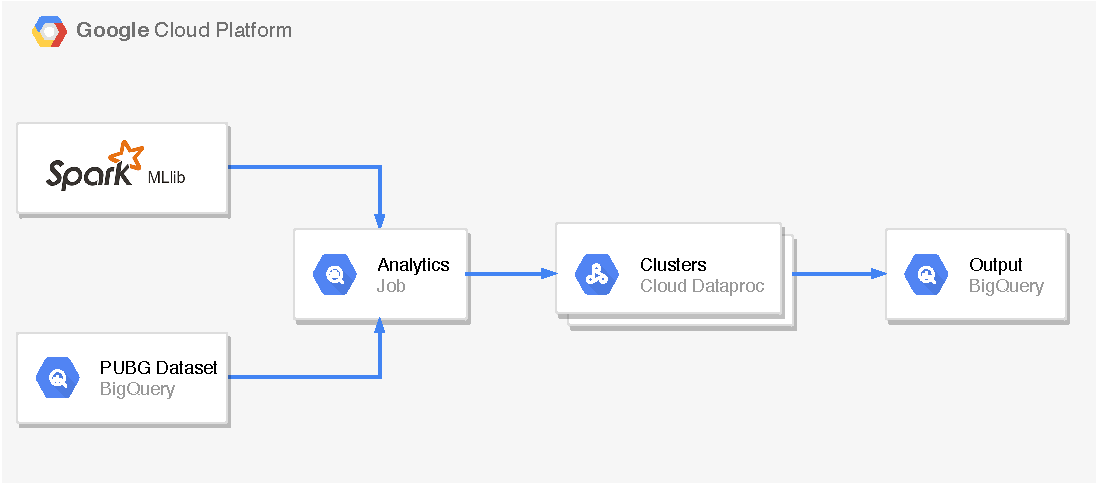
\includegraphics[width=9cm]{images/flow.pdf}
  \caption{Workflow of the analytics operation which is described in the Implementation section \ref{sec:implementation}.}
  \label{fig:1}
\end{figure}

\section{Algorithms}
\label{sec:algorithms}
Algorithms used in this report are for prediction of the win placement percentile of a given player. We have used regression algorithms, AdaBoost Regressor, Gradient Boosting Regressor, Random Forest Regressor and Decision Tree Regressor.

\subsection{AdaBoost Regressor}
AdaBoost, also known as Adaptive Boosting, is one of the first boosting algorithms proposed by Gödel Prize winners Robert E. Schapire and Yoav Freund in 2012 in their published book "Boosting: Foundations and Algorithms"~\cite{schapire_boosting_2012}. 

A boosting algorithm works by combining multiple weak algorithms which have no correlations amongst each other and voting for the best solution. In this way, a couple of weak algorithms come together to make one strong algorithm. Boosting algorithms are based on ensemble learning, which literally means "a group producing a single effect".

AdaBoost uses decision tree with a single split as its weak algorithm often called as decision stumps and applies boosting over it. Since AdaBoost is based on ensemble learning, it tries to fit all data points, it fails with noisy data. The most astonishing thing about this algorithm is that it does not overfits even though it is trying to fit all the data points. AdaBoost Regressor can be used both for classification and regression problems.

\subsection{Gradient Boosting Regressor}
Similarly to AdaBoost discussed earlier, gradient boost is also an ensemble learning based boosting algorithm. It also works on decision stumps. This algorithm was proposed by Friedman in 1999 in his paper titled "Greedy Function Approximation: A Gradient Boosting Machine"~\cite{friedman_greedy_2001}. The only difference between AdaBoost and gradient boost is that depth level of the tree varies from 8 to 32 in the latter while the depth level is 1 in the former. This algorithm can also be applied for solving classification and regression problems.

\subsection{Random Forest Regressor}
Ho discovered this supervised learning algorithm in 1995~\cite{tin_kam_ho_random_1995}. Random forest is also based on ensemble learning similarly to AdaBoost and gradient boost. There are two types of ensemble learnings, boosting and bagging. Unlike AdaBoost and gradient boost, random forest is a bagging based technique. Bagging also referred to as bootstrap aggregating which samples data randomly with a possibility of replacement. This technique enables multiple models to operate without intervening with each other.

In the random forest algorithm based on bagging, all its trees run independetly together. These trees are decision trees generated during training. The benefit of this algorithm is that it can swiftly handle large amount of data but it overfits with noisy data.

\subsection{Decision Tree Regressor}
Decision tree is a predictive modelling algorithm which with the help of a collection of binary rules predict an output. These rules are formed by a QnA by the algorithm on the data to narrow down to the problem until it reaches a final conclusion. It can be used for both classification and regression problems. But this algorithm is not suitable for continuous variables and is also prone to over fitting.

In this report, we will be using the above mentioned algorithms to perform our primary goal of predicting win placement percentile of players. These algorithms will be compared on the basis of their accuracy.

\section{Implementation}
\label{sec:implementation}
The code of this report has been implemented in python using APIs of Apache Spark's machine learning library, PySpark. This library specifically for python to use Apache Spark's resources on a cluster. The code uses python 3.7.0. The program workflow as shown in figure \ref{fig:1}, relies on GCP for data storage as well as Apache Spark clusters.

The data is stored in BigQuery which is used for storing large amounts of data both streaming as well as non-streaming. BigQuery provides prallel processing of SQL queries on a large scale and outputs result in fraction of seconds. This is why BigQuery has been selected as an ideal data hosting service. The data from BigQuery is fed to our program where it is stored as RDD (Resilient Distributed Dataset). Since we had to do some pre-processing of the data, we converted the data to Pandas Dataframe so that we can utilise its APIs. This pre-processed data is then stored in BigQuery so that we won't have to perform pre-processing everytime our cluster runs the program thus preventing huge bills.

This newly stored pre-processed data is then used by our main program where multiple supervised learning algorithms are applied on it to get predictions. This program is then deployed on a cluster running on Dataproc.

In the following sections, each of the steps defined above is described briefly.

\subsection{Data Pre-processing}
The original dataset had 29 variables. A few of them were categorical variables rest were numerical continuous variables. The following categorical variables were dropped from the dataset which seemed to be not much useful:

\begin{table}[h]
    \caption{Categorical variables which were dropped}
    \label{tab:cat_variables}
	\centering
    \begin{tabular}{l l l}
    \toprule
    \multirow{2}{*}{Variable} & \multirow{2}{*}{Description} & \multirow{2}{*}{Sample Data} \\ 
    && \\ \midrule
    $Id$ & Player's unique identifier & 7f96b2f878858a \\ \midrule
    $matchId$ & Unique identifier for matches & a10357fd1a4a91 \\ \midrule
    $groupId$ & Unique identifier for groups in a match & 4d4b580de459be  \\
    \bottomrule
    \end{tabular}
\end{table}

We then converted the column $matchType$ from categorical variable to numerical variable, resulting in 15 categories. Since some matches did not had 100 players, we cannot compare data of different matches as the number of players is not same in both, so we normalized the $kills$ and $damageDealt$ variables. To normalize them, we used the formulaes given below:

\[ killsNorm = \frac{kills}{totalPlayers} * 100 \]

\[ damageDealtNorm = \frac{damageDealt}{totalPlayers} * 100 \]

We then created another normalized variable, $normMatchType$ with $matchType$ values. Due to huge differences in the size of the solo game or of a team game, we set this 'other' and to the normal team size: 1 for solo; 2 for a double; < 4 for the team; and other for the rest. The data are different from the standard team sizes. Data from the custom games are also made up of different values of team sizes like 10, 15, 92, etc. that are added to a different value.

We then did feature engineering where we created 13 additional variables:

\subsubsection{totalDistance}
$totalDistance$ is calculated by summing up $rideDistance$, $walkDistance$ and $swimDistance$.

\subsubsection{maxPossibleKills}
$maxPossibleKills$ is the maximum kills a player can do in a match which is calculated using $totalPlayers - teamSize$.

\subsubsection{itemsUsed}
$itemsUsed$ is all the items the player has picked up or used. Items which we have data of are $boosts$, $heals$ and $weaponsAcquired$.

\subsubsection{itemsPerDistance}
$itemsPerDistance$ is the normalized value of $\frac{itemsUsed}{totalDistance}$.

\subsubsection{killsPerDistance}
$killsPerDistance$ is the normalized value of $\frac{kills}{totalDistance}$.

\subsubsection{damageDealtPerDistance}
$damageDealtPerDistance$ is the normalized value of $\frac{damageDealt}{totalDistance}$.

\subsubsection{maxTeamKills}
$maxTeamKills$ shows the maximum number of team kills a player has done.

\subsubsection{totalTeamKills}
$totalTeamKills$ is the total kills a team has performed together.

\subsubsection{headshotKillRate}
$headshotKillRate$ is made for identifying the skill of the player by dividing total number of headshot kills he did, $headshotKills$ by the total $kills$.

\subsubsection{itemsUsedPerTeam}
$itemsUsedPerTeam$ is the total number of items used by a team combined.

\subsubsection{percKill}
$percKill$ is the percentage of kills a player has performed in a match based on the maximum kills a player can do in a match.

\subsubsection{percTeamKills}
$percTeamKills$ is the percentage of kills a team has performed in a match based on the maximum kills a team can do in a match.

\subsubsection{meanTeamKillPlace}
$meanTeamKillPlace$ is the mean of $killPlace$ for all players in the team.

This data is now ready for applying our machine learning algorithms and is stored in BigQuery.

\subsection{Applying Machine Learning Algorithms}
The above processed data is now fetched in our main PySpark program which will run on cluster for predictions. While fetching this data, the library somehow interprets the variables as $object$ type rather than numeric. So we have to convert these values to numeric value with the below code:

\begin{lstlisting}[language=Python]
for col in cols:
    pubg = pubg.withColumn(col, pubg[col].cast(FloatType()))
\end{lstlisting}

The algorithms applied on the data are AdaBoost, Gradient Boost, Random Forest and Decision Tree. $learning_rate$ has been choosen 80\% for AdaBoost and Gradient Boost while $n\_estimators$ is 10 for Random Forest. The code is shown below for the algorithms applied:

\begin{lstlisting}[language=Python]
model_1 = AdaBoostRegressor(learning_rate=0.8)
model_1.fit(X_train,y_train)

model_2 = GradientBoostingRegressor(learning_rate=0.8)
model_2.fit(X_train,y_train)

model_3 = RandomForestRegressor(n_estimators=10)
model_3.fit(X_train,y_train)

model_4 = DecisionTreeRegressor()
model_4.fit(X_train,y_train)
\end{lstlisting}

\subsection{Deploying the program to Dataproc cluster}
Now this program is ready for deploying it on the Apache Spark cluster. Before deploying it to the cluster, the cluster needs to be setup from Google Cloud Console or using $gcloud$ cli command.

The following figure \ref{fig:2} shows a screen capture of the Dataproc where it is showing inputs for clusters formation.
\begin{figure}[h]
    \centering
    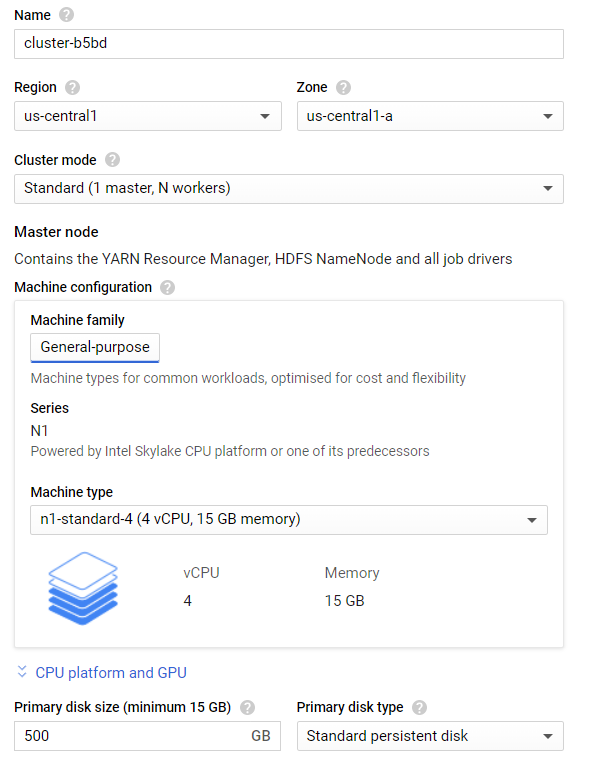
\includegraphics[scale=0.65]{images/cluster_1.png}
    \caption{Google Cloud Console screen of cluster creation}
    \label{fig:2}
\end{figure}

\newpage

Alternatively, we can create a cluster using $gcloud$ cli.

\begin{lstlisting}
    $ gcloud dataproc clusters create cluster-b5bd --region us-central1 --subnet default --zone us-central1-a --master-machine-type n1-standard-4 --master-boot-disk-size 500 --num-workers 2 --worker-machine-type n1-standard-4 --worker-boot-disk-size 500 --image-version 1.3-deb9 --project lyit
\end{lstlisting}

The parameters we used for creating clusters are:
\begin{table}[h]
    \caption{Google Cloud Dataproc parameters for cluster}
    \label{tab:parameters}
	\centering
    \begin{tabular}{l l}
    \toprule
    \multirow{1}{*}{Parameter} & \multirow{1}{*}{Value} \\ 
    & \\ \midrule
    Region & us-central1 (default) \\ \midrule
    Subnet & default \\ \midrule
    Subnet zone & us-central1-a \\ \midrule
    Master machine type & n1-standard-4 \\ \midrule
    Master boot disk size & 500 GB \\ \midrule
    Workers & 2 \\ \midrule
    Worker machine type & n1-standard-4 \\ \midrule
    Worker boot disk size & 500 GB \\ \midrule
    Image version & 1.3-deb9 \\
    \bottomrule
    \end{tabular}
\end{table}

\subsection{Visualizing the output}
Some of the visualizations have been directly done on Jupyter notebook but most of the visualizations have been done on Google Data Studio which gives a connector to BigQuery and gives flexibility for visualizing large volumes of data.

\section{Experimentation Results and Discussions}
\label{sec:discussion}
In this section we will be looking at the results of our program and answer the questions which we set out with earlier in the introduction section \ref{sec:introduction}.

\subsection{Average time a player spends in a match}
Using $matchDuration$ variable, we have calculated the average time a player spends in a match.

The average time is {1579.51 seconds which translates to 26.32 minutes. 

\subsection{Total number of kills done by users when playing alone versus when playing in a team}
The following figure \ref{fig:3} shows the share of users performing kills in different $matchType$ scenarios.

\begin{figure}[h]
    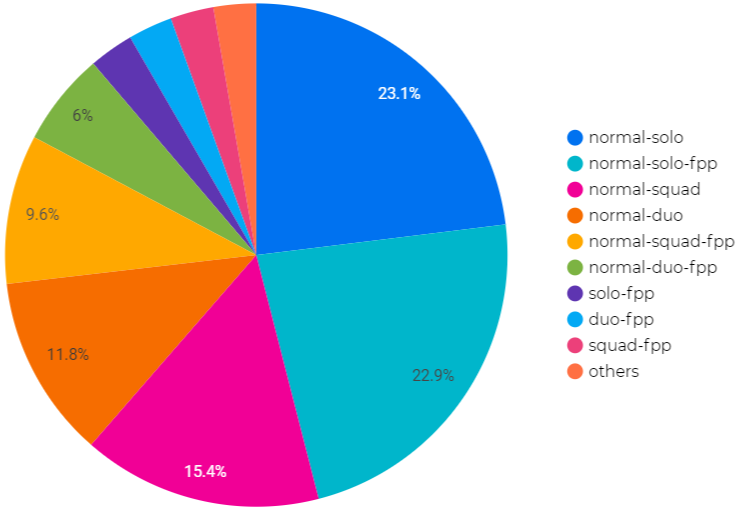
\includegraphics[width=9cm]{images/match_type_vs_kills.png}
    \caption{Kills done by users when playing alone versus when playing in team}
    \label{fig:3}
\end{figure}

From the figure, it can be noted that solo players perform most kills rather than team players. Around 50\% of kills are performed by solo players.

\subsection{How better a player performs (in terms of $rankPoints$, $winPlace$, $winPoints$) when playing alone versus when playing in a team?}

\begin{table}[h]
    \caption{Player performance in terms of $rankPoints$, $winPlace$, $winPoints$ when playing alone versus when playing in a team}
    \label{tab:player_performance}
	\centering
    \begin{tabular}{l l l l}
    \toprule
    \multirow{1}{*}{Game Type} & \multirow{1}{*}{rankPoints} & \multirow{1}{*}{winPlacePerc} & \multirow{1}{*}{winPoints} \\ 
    &&& \\ \midrule
    Team & 772.25585284 & 0.592398494983 & 736.991638795 \\ \midrule
    Solo & 759.890547263 & 0.691486069651 & 779.452736318 \\
    \bottomrule
    \end{tabular}
\end{table}


\begin{table}[h]
    \caption{Performance of different algorithms run on the same dataset}
    \label{tab:summary}
	\centering
    \begin{tabular}{l l l}
    \toprule
    \multirow{1}{*}{Algorithm} & \multirow{1}{*}{Category} & \multirow{1}{*}{Accuracy} \\ 
    && \\ \midrule
    AdaBoost Regressor & Ensemble Learning Boosting & 91.71\% \\ \midrule
    Gradient Boosting Regressor & Ensemble Learning Boosting & 94.86\% \\ \midrule
    Random Forest Regressor & Ensemble Learning Boosting & 93.97\% \\ \midrule
    Decision Tree Regressor & - & 81.58\% \\
    \bottomrule
    \end{tabular}
\end{table}

\section{Conclusion}
\label{sec:conclusion}

\bibliographystyle{IEEEtran}
\bibliography{bib}

\end{document}
